\section{Attività ottica}
Una delle proprietà più importanti degli enantiomeri è la loro capacità di far ruotare sul piano della luce polarizzata. Per questo motivo gli enantiomeri si definiscono \textbf{otticamente attivi}.

\paragraph{Ma cos'è la luce polarizzata?} Sappiamo che la luce è composta da onde che oscillano in tutti i piani perpendicolari alla sua direzione di propagazione. Tramite alcuni materiali si può isolare una sola onda della luce che oscilla in un solo piano, questa onda viene chiamata \textbf{luce piano-polarizzata}.

\subsection{Polarimetro}
La luce polarizzata è in grado di attraversare due materiali polarizzatori soltanto se i loro assi di polarizzazione sono allineati; se invece sono perpendicolari la luce non passa. Questo è su cui si basa il \textbf{polarimetro}, lo strumento che serve per studiare l'effetto delle sostanze sulla luce polarizzata.

\paragraph{Funzionamento del polarimetro}\mbox{}\\
Con la sorgente luminosa accesa e il tubo portacampioni vuoto, il prisma analizzatore viene ruotato in modo che il campo visivo dell'osservatore risulti oscurato. Gli assi del prisma polarizzatore e del prisma analizzatore sono perpendicolari tra loro.

Ora il campione da analizzare viene inserito all'interno del tubo portacampioni. Se la sostanza da analizzare è \textbf{otticamente inattiva}, non farà ruotare il piano della luce polarizzata e il campo visivo dell'osservatore continuerà ad essere nero.
Se la sostanza invece è \textbf{otticamente attiva}, il piano della luce polarizzata subirà una rotazione e un po' di luce giungerà all'occhio dell'osservatore.

\begin{figure}[htp]
	\centering
	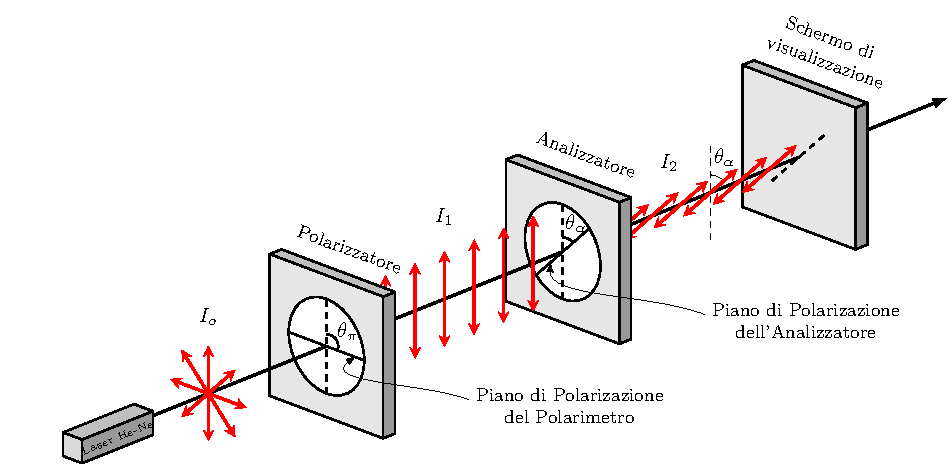
\includegraphics{Capitoli/Stereoisomeria/grafici/polarimetro.pdf}
	\caption{Schema di un polarimetro}
\end{figure}

L'asse del prisma analizzatore dovrà essere ruotato di un certo angolo \(\alpha\) per rendere il campo visivo nuovamente nero.
L'angolo \(\alpha\) viene detto \textbf{rotazione osservata} e corrisponde all'entità della rotazione della luce polarizzata.

Se l'analizzatore deve essere ruotato a destra, la sostanza è detta \textbf{destrorotatoria} e indicata con \iupac{(+)}; mentre se viene girato a sinistra, la sostanza è detta \textbf{levorotatoria} e indicata con \iupac{($-$)}.


La rotazione osservata, \(\alpha\), di un campione dipende da diversi fattori:
\begin{itemize}
	\item struttura molecolare
	\item numero di molecole all'interno del tubo portacampioni
	\item lunghezza del tubo
	\item lunghezza d'onda della luce polarizzata
	\item temperatura
\end{itemize}

La \textbf{rotazione specifica}, \(\left[\alpha\right]\), è definita come la rotazione osservata per una specifica lunghezza della cella e una specifica concentrazione del campione.
\begin{equation*}
	\text{Rotazione specifica} = \left[\alpha\right]^{T}_{\lambda} = \frac{\alpha}{l\times c} (\text{solvente}) = \frac{\text{Rotazione osservata (gradi)}}{\text{Lunghezza (\unit{\dm})} \times \text{Concentrazione}}
\end{equation*}

Il solvente viene sempre indicato tra parentesi. Le misure vengono effettuate in genere a temperatura ambiente (\unit{25\celsius}) e la fonte di luce più comune è la riga D del sodio (\(\lambda = \unit{593,3\nm}\)).


